\section{Pembuktian Hipotesis}
\label{sec:bukti-hipotesis}

Dugaan awal yang mendasari penelitian ini adalah pemasokan BBM di Kabupaten Maluku Barat Daya belum optimal karena kapal yang digunakan tidak mampu beropeasi pada saat gelombang tinggi.

\subsection{Pengaruh Ukuran Utama terhadap Operasional Kapal}
\label{subsec:ukuran-vs-operasional}

Langkah awal yang dilakukan adalah membuktikan bahwa ukuran kapal berpengaruh terhadap kemampuan operasional pada ketinggian gelombang tertentu. Pengujian dilakukan dengan dasar model lambung kapal \emph{ship pro} yang disertakan pada perangkat lunak \emph{Maxsurf}. Lambung kapal tersebut kemudian diskalakan dan diuji kemampuan olah geraknya dalam \emph{Maxsurf Motions}. Hasil uji olah gerak kemudian dievaluasi berdasarkan kriteria yang sudah dibahas pada bab \ref{subsec:kriteria-seakeeping}.

\begin{table}[!ht]
    \centering
    \caption{Ukuran Kapal yang Dievaluasi}
    \label{tab:variasi-ship-dimensions}
    \begin{tabular}{|l|l|l|l|l|}
    \hline
    Ship Name & L 76  & L 60  & L 50 & L 40 \\ \hline
    Lpp [m]      & 76,8  & 60    & 50   & 40   \\ \hline
    Beam [m]      & 13,50 & 10,55 & 8,79 & 7,03 \\ \hline
    Depth [m]    & 7,75  & 6,05  & 5,05 & 4,04 \\ \hline
    Draft [m]    & 4,57  & 3,57  & 2,98 & 2,38 \\ \hline
    \end{tabular}
\end{table} 

\begin{figure}[!ht]
    \centering
    % First row - two images side by side
    \begin{subfigure}{0.48\textwidth}
        \centering
        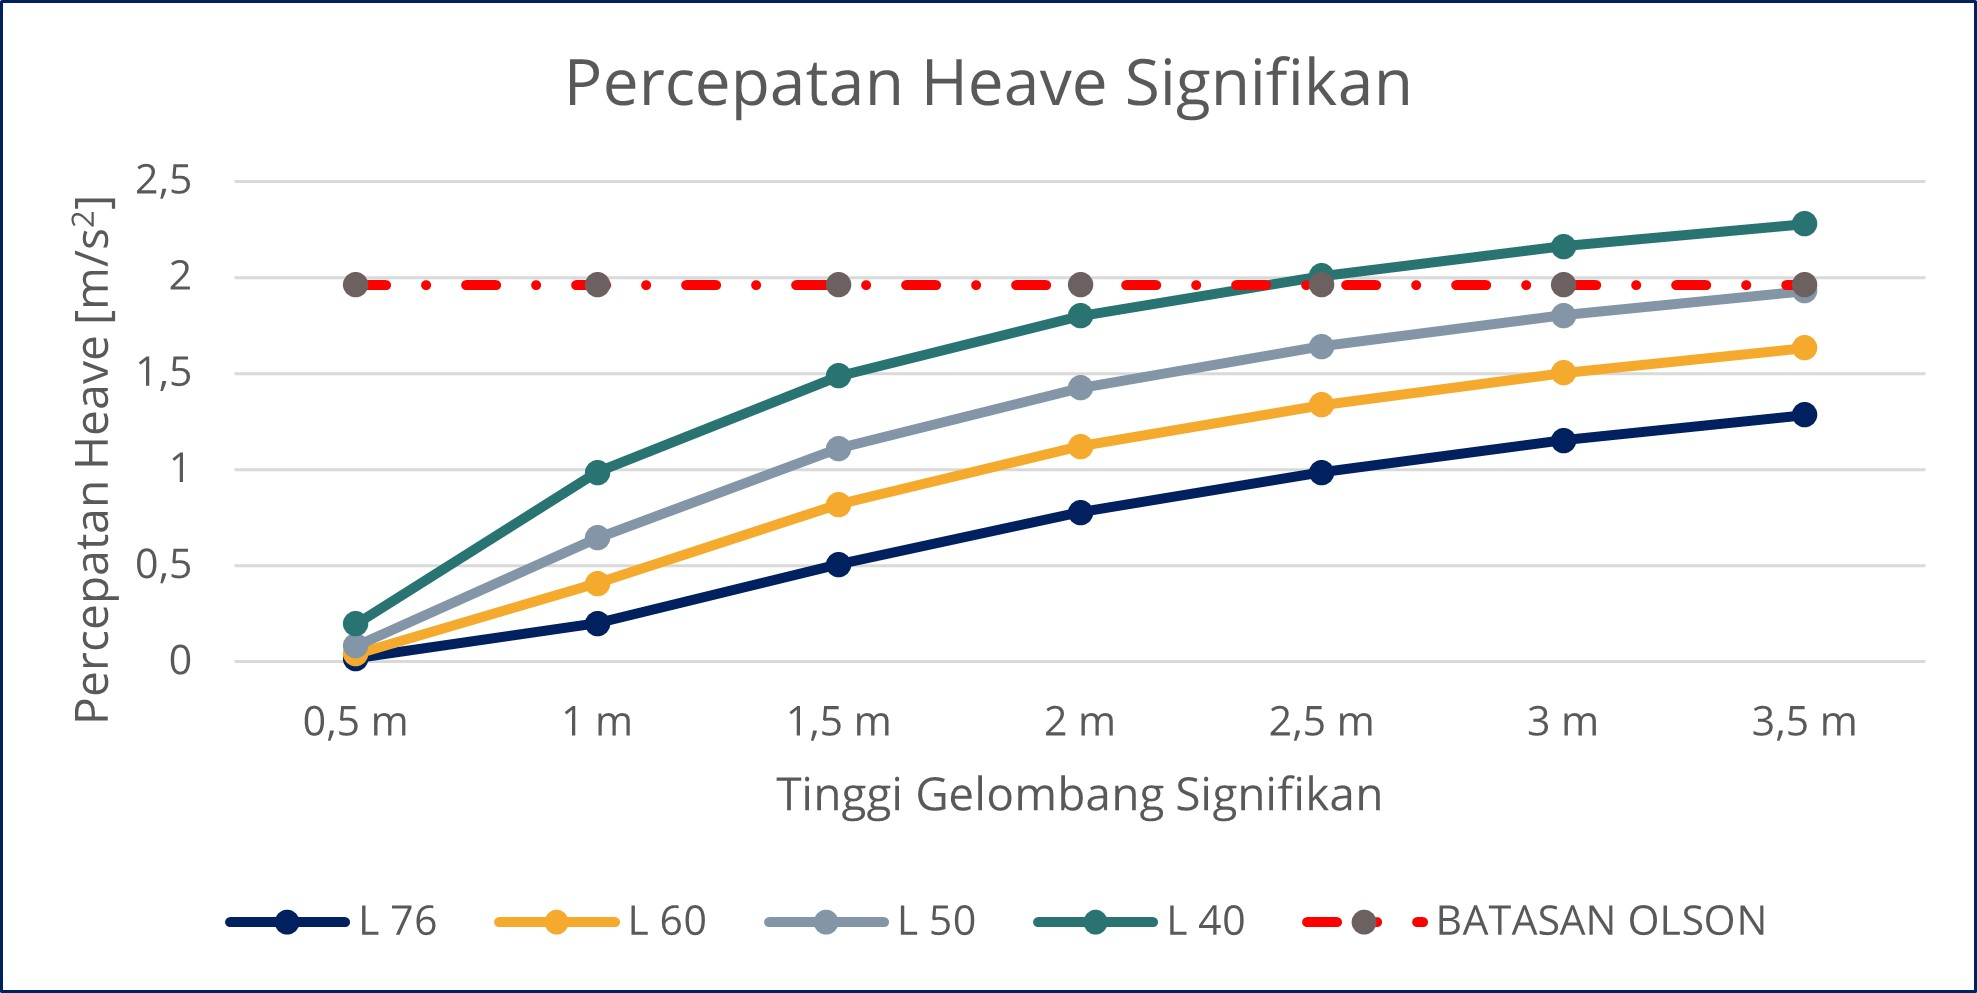
\includegraphics[width=\textwidth]{grafik/uji-heave-ori.jpg}
        \caption{Hasil Uji Gerak \emph{Heave}}
        \label{fig:uji-heave-ori}
    \end{subfigure}
    \hfill
    \begin{subfigure}{0.48\textwidth}
        \centering
        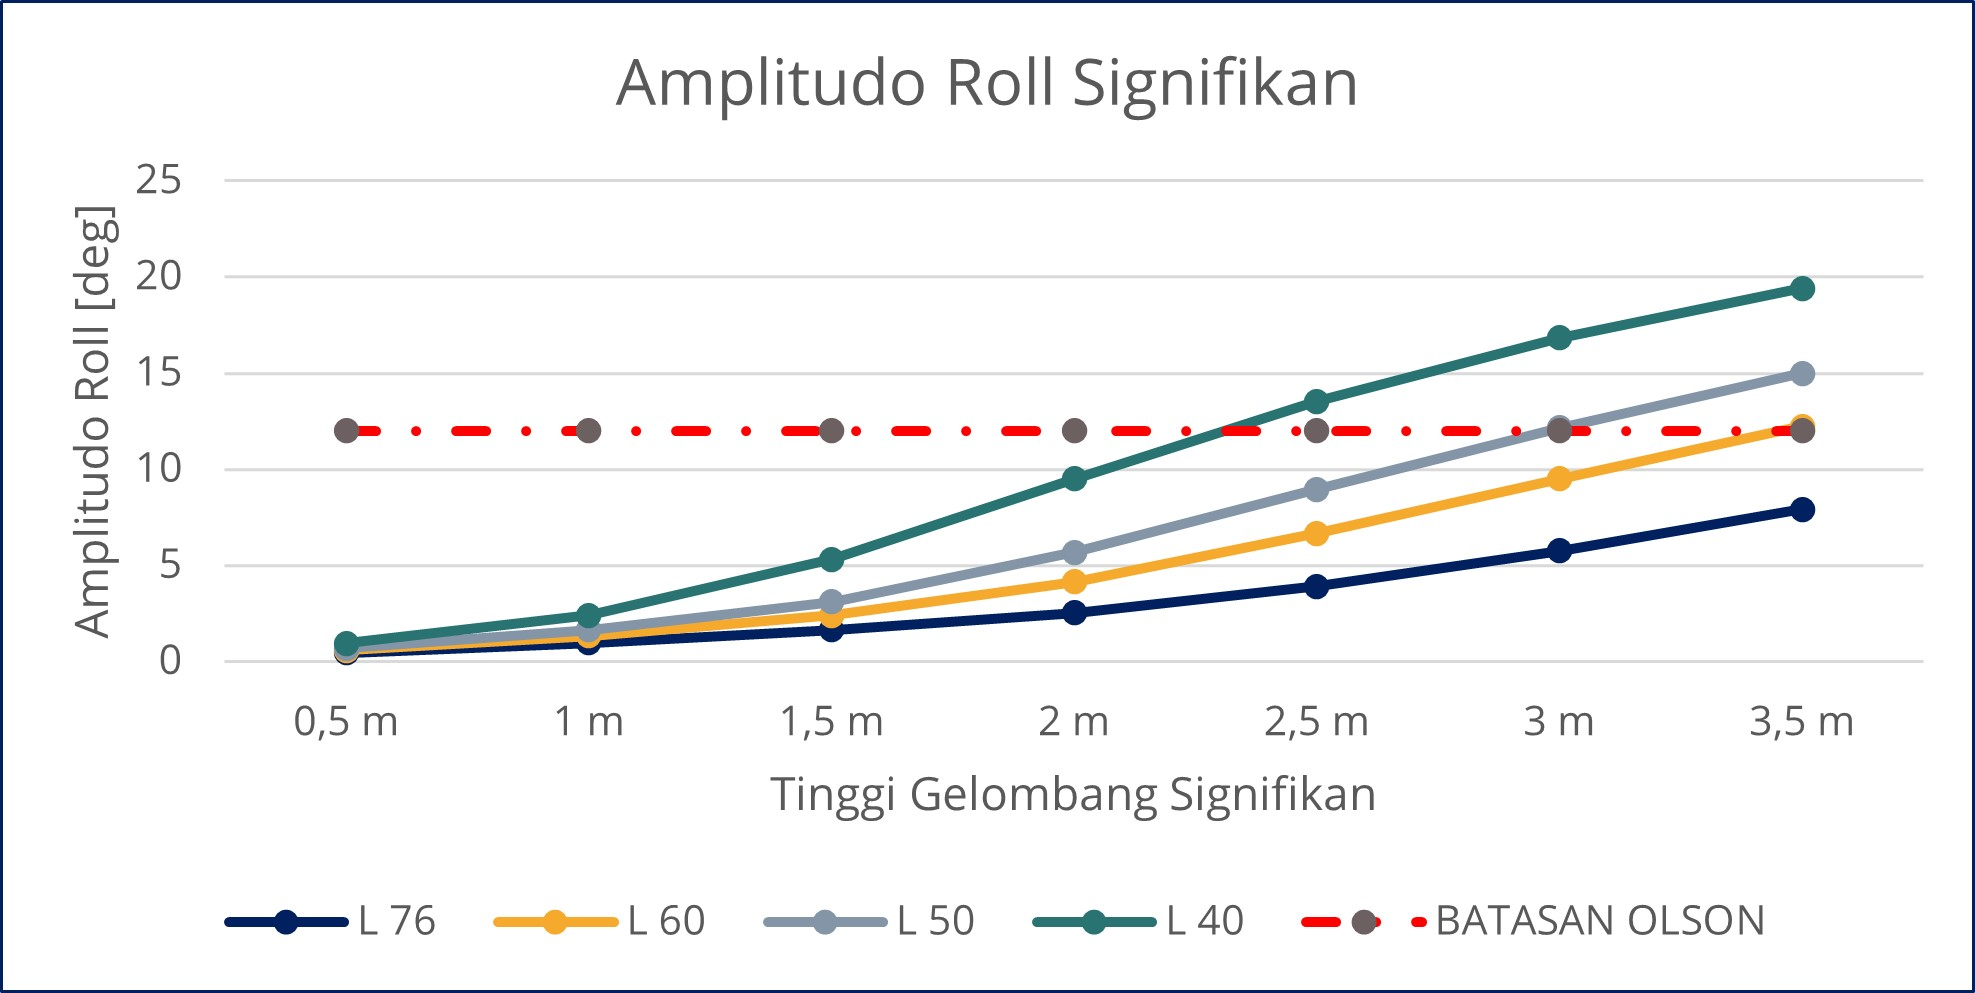
\includegraphics[width=\textwidth]{grafik/uji-roll-ori.jpg}
        \caption{Hasil Uji Gerak \emph{Roll}}
        \label{fig:uji-roll-ori}
    \end{subfigure}
    
    \vspace{1cm}  % Add vertical space between rows
    
    % Second row - single image centered
    \begin{subfigure}{0.48\textwidth}
        \centering
        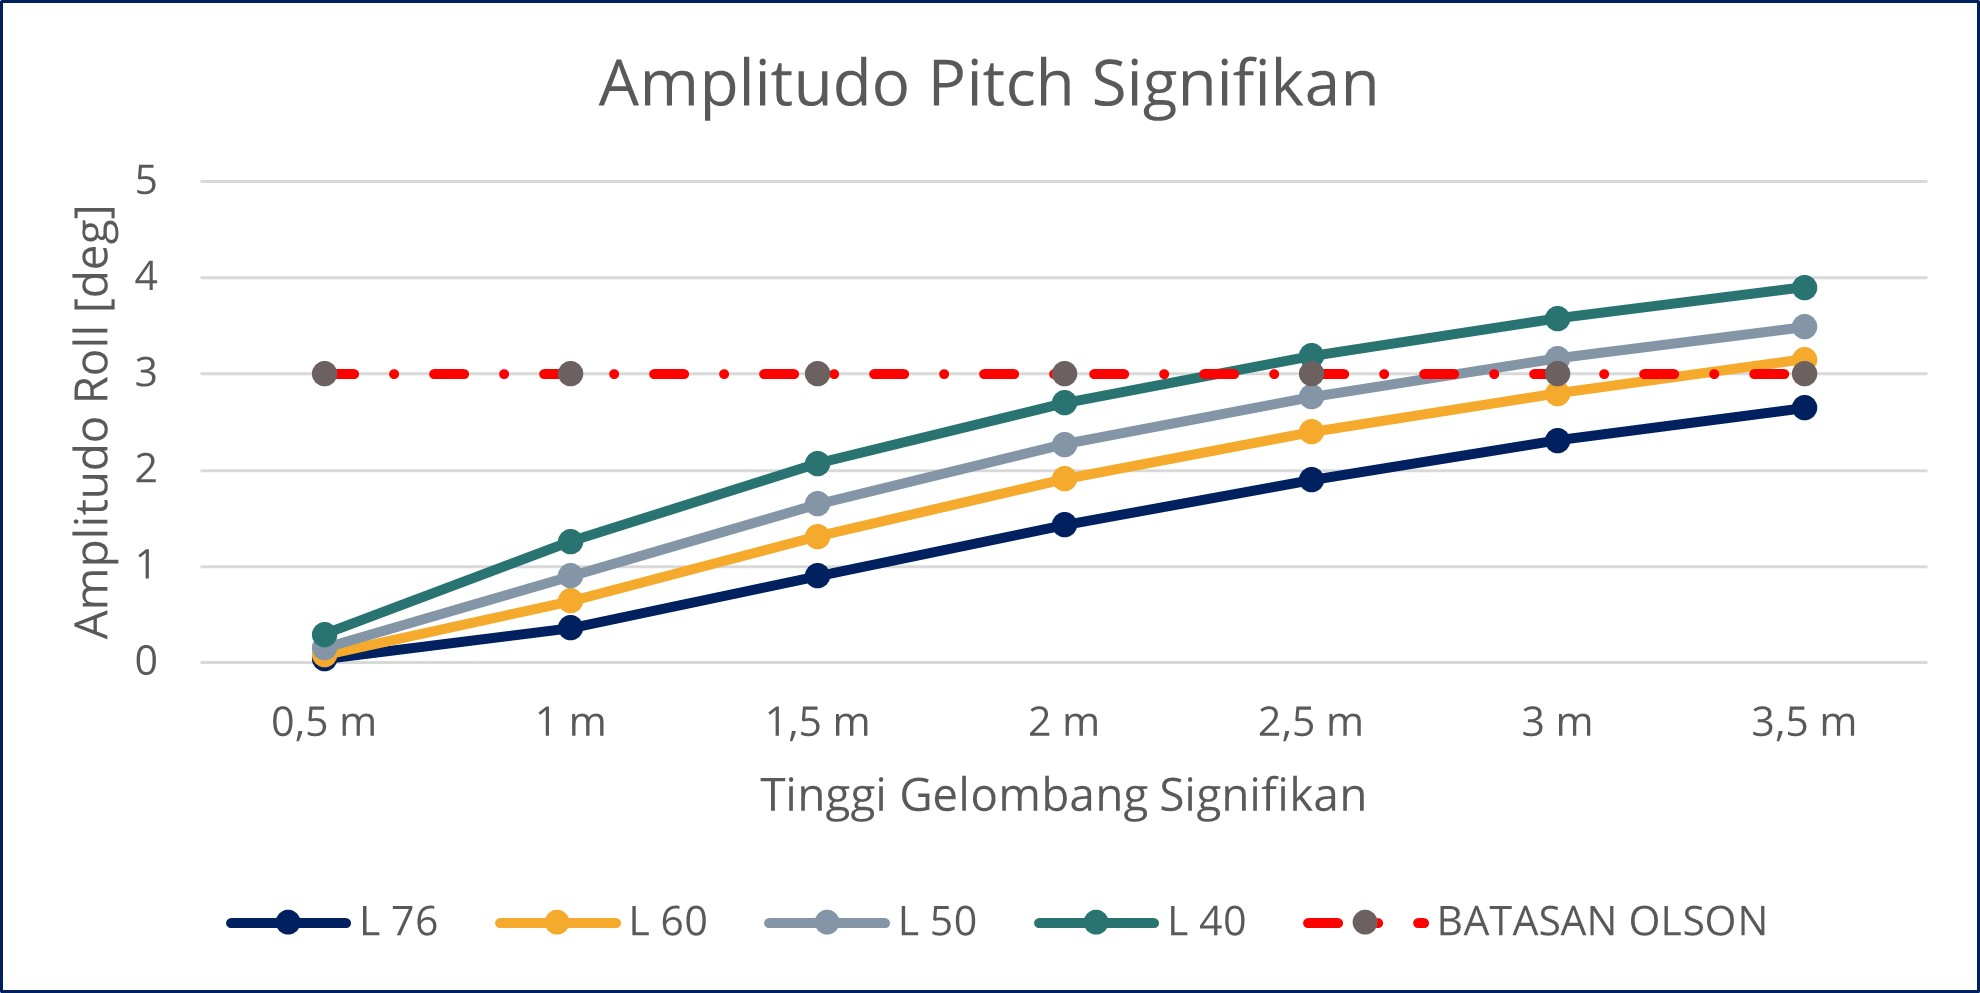
\includegraphics[width=\textwidth]{grafik/uji-pitch-ori.jpg}
        \caption{Hasil Uji Gerak \emph{Pitch}}
        \label{fig:uji-pitch-ori}
    \end{subfigure}
    \caption{Hasil Uji \emph{Seakeeping} Model Kapal}
    \label{fig:uji-gerak-all}
\end{figure}
% \begin{figure}[!ht]
%     \centering
%     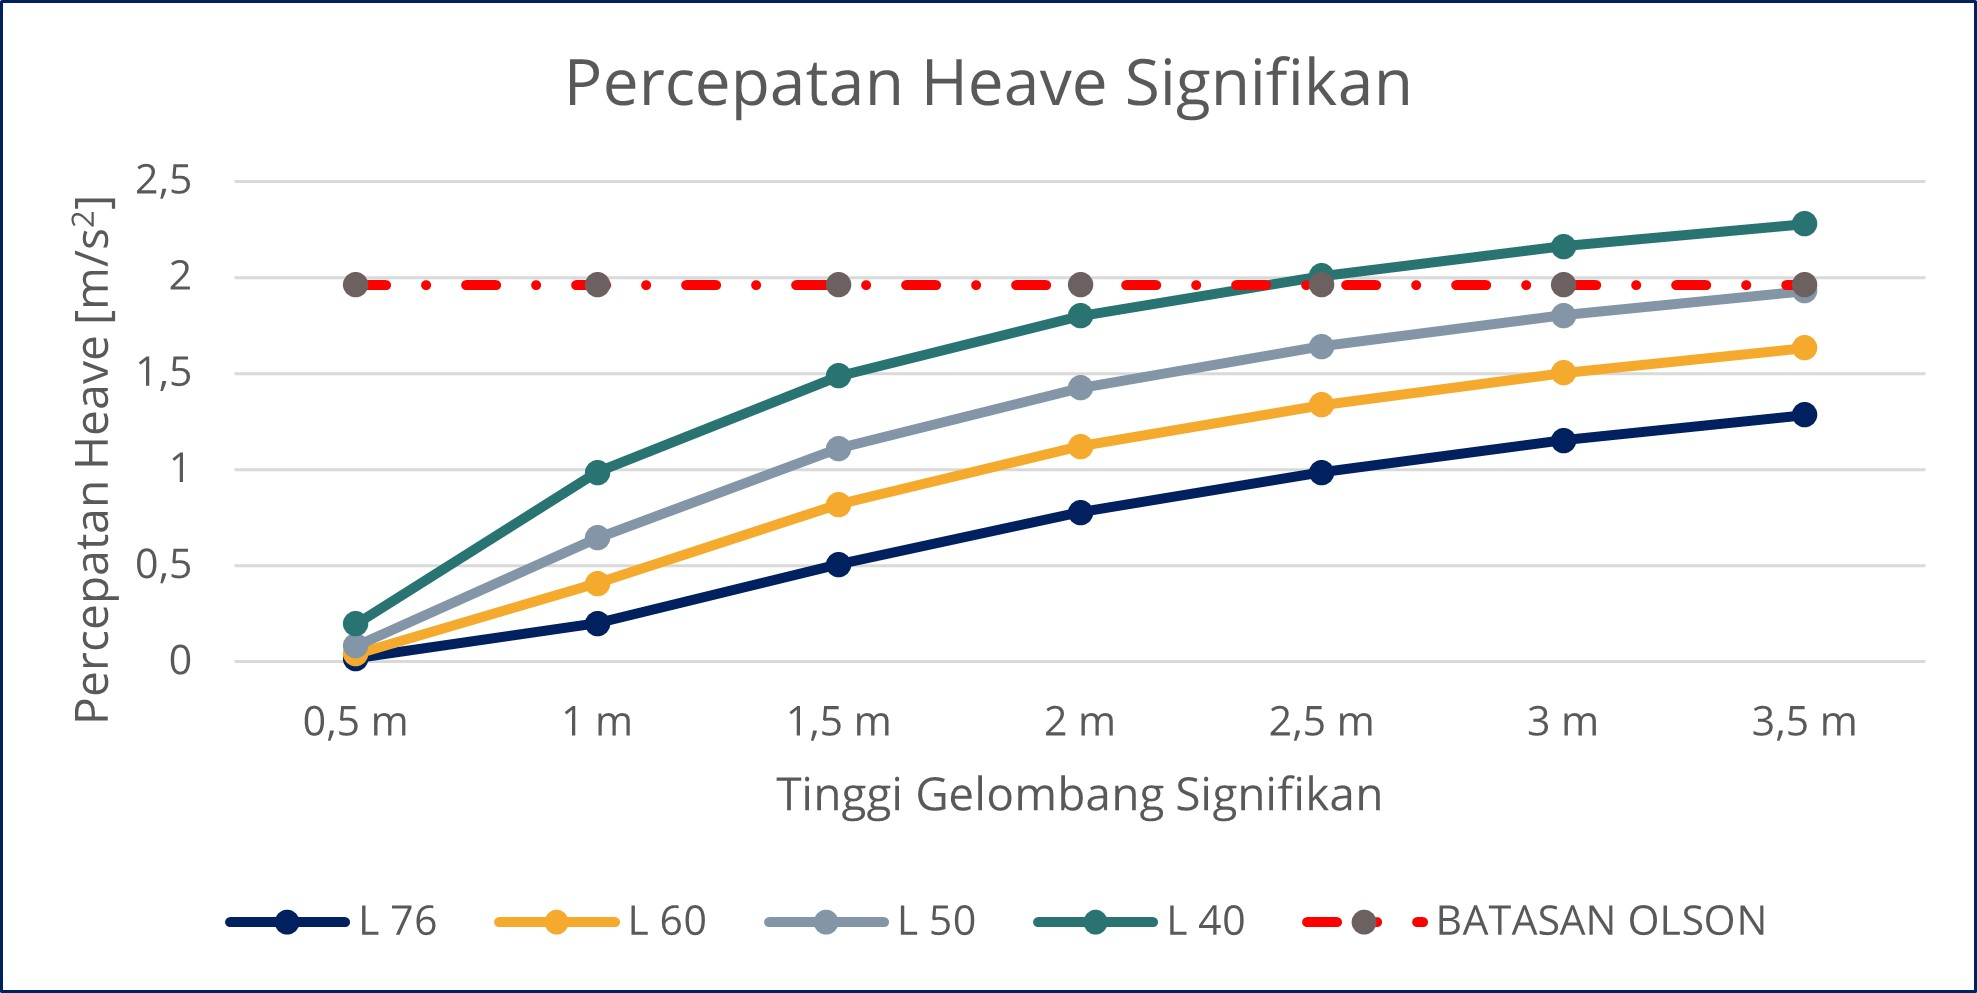
\includegraphics[width=0.65\textwidth]{grafik/uji-heave-ori.jpg}
%     \caption{Hasil Uji Gerak \emph{Heave}}
%     \label{fig:uji-heave-ori}
% \end{figure}

% \begin{figure}[!ht]
%     \centering
%     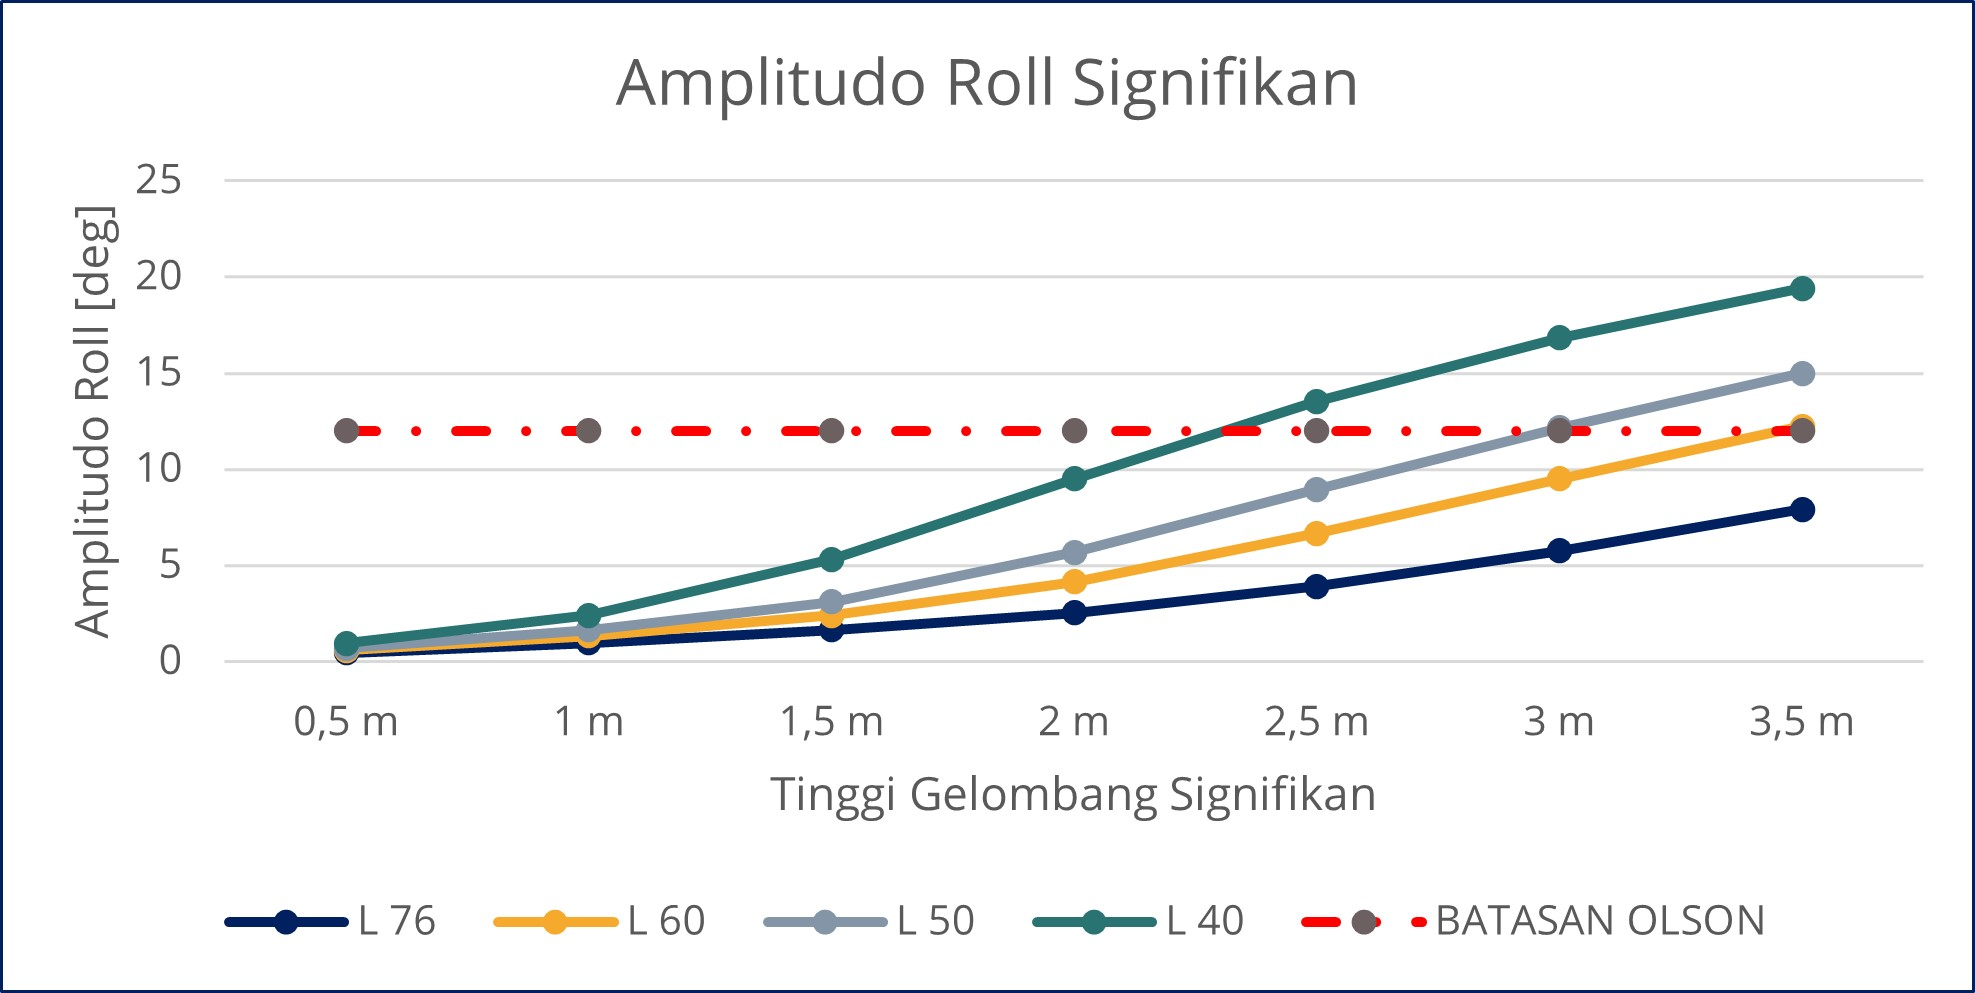
\includegraphics[width=0.65\textwidth]{grafik/uji-roll-ori.jpg}
%     \caption{Hasil Uji Gerak \emph{Roll}}
%     \label{fig:uji-roll-ori}
% \end{figure}

% \begin{figure}[!ht]
%     \centering
%     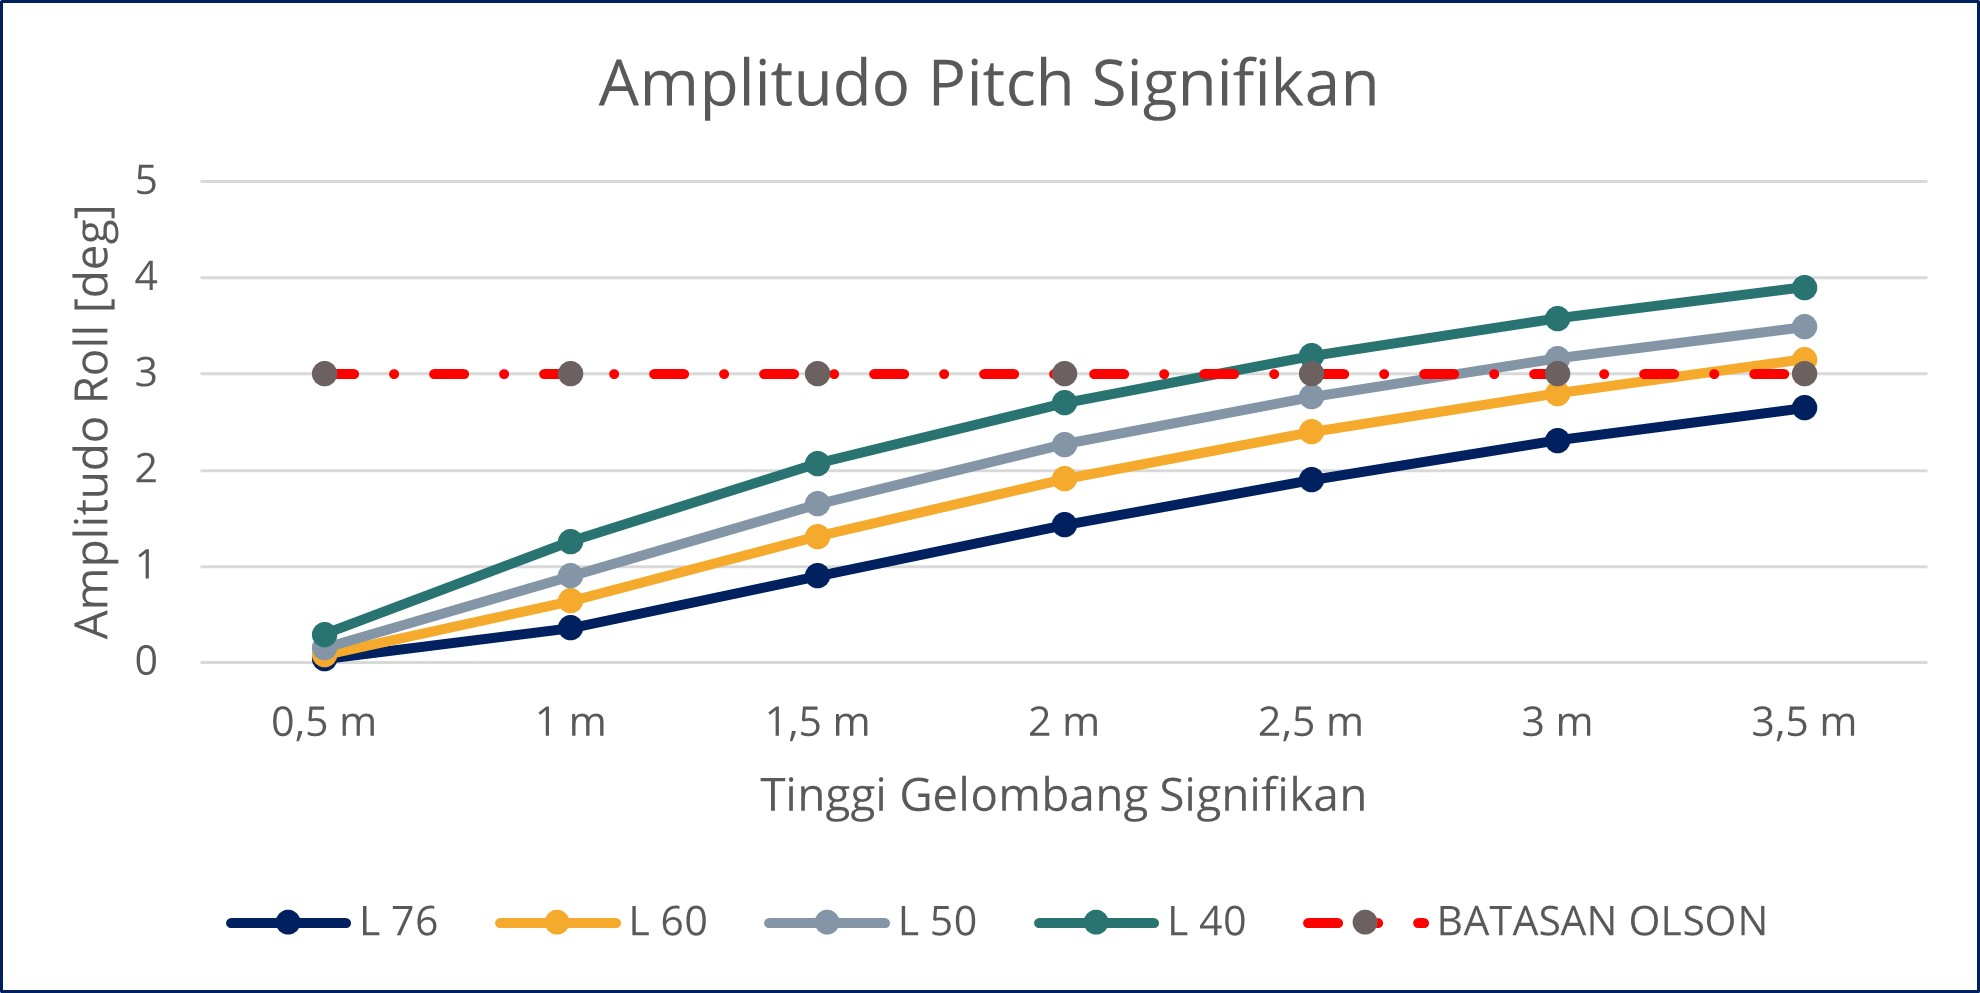
\includegraphics[width=0.65\textwidth]{grafik/uji-pitch-ori.jpg}
%     \caption{Hasil Uji Gerak \emph{Pitch}}
%     \label{fig:uji-pitch-ori}
% \end{figure}

Dapat dilihat pada gambar \ref{fig:uji-heave-ori} hingga \ref{fig:uji-pitch-ori} bahwa semakin besar ukuran kapal semakin tahan terhadap gangguan kapal. Hasil ini akan dijadikan pertimbangan dalam merancang kapal baru.

\subsection{Hasil Uji \emph{Seakeeping}}
\label{subsec:hasil-uji-seakeeping}

Penentuan batas ketinggian gelombang dimana kapal yang sudah ada saat ini dapat beroperasi dilakukan dengan cara menguji kemampuan olah gerak kapal yang sudah ada saat ini dengan gelombang yang mungkin muncul di jalur pemasokan BBM Kabupaten MBD. Pengujian dilakukan dengan dua variasi kecepatan (5 dan 6 knot) dan garis air setinggi 2 meter.

\begin{figure}[!ht]
    \centering
    \begin{subfigure}{0.48\textwidth}
        \centering
        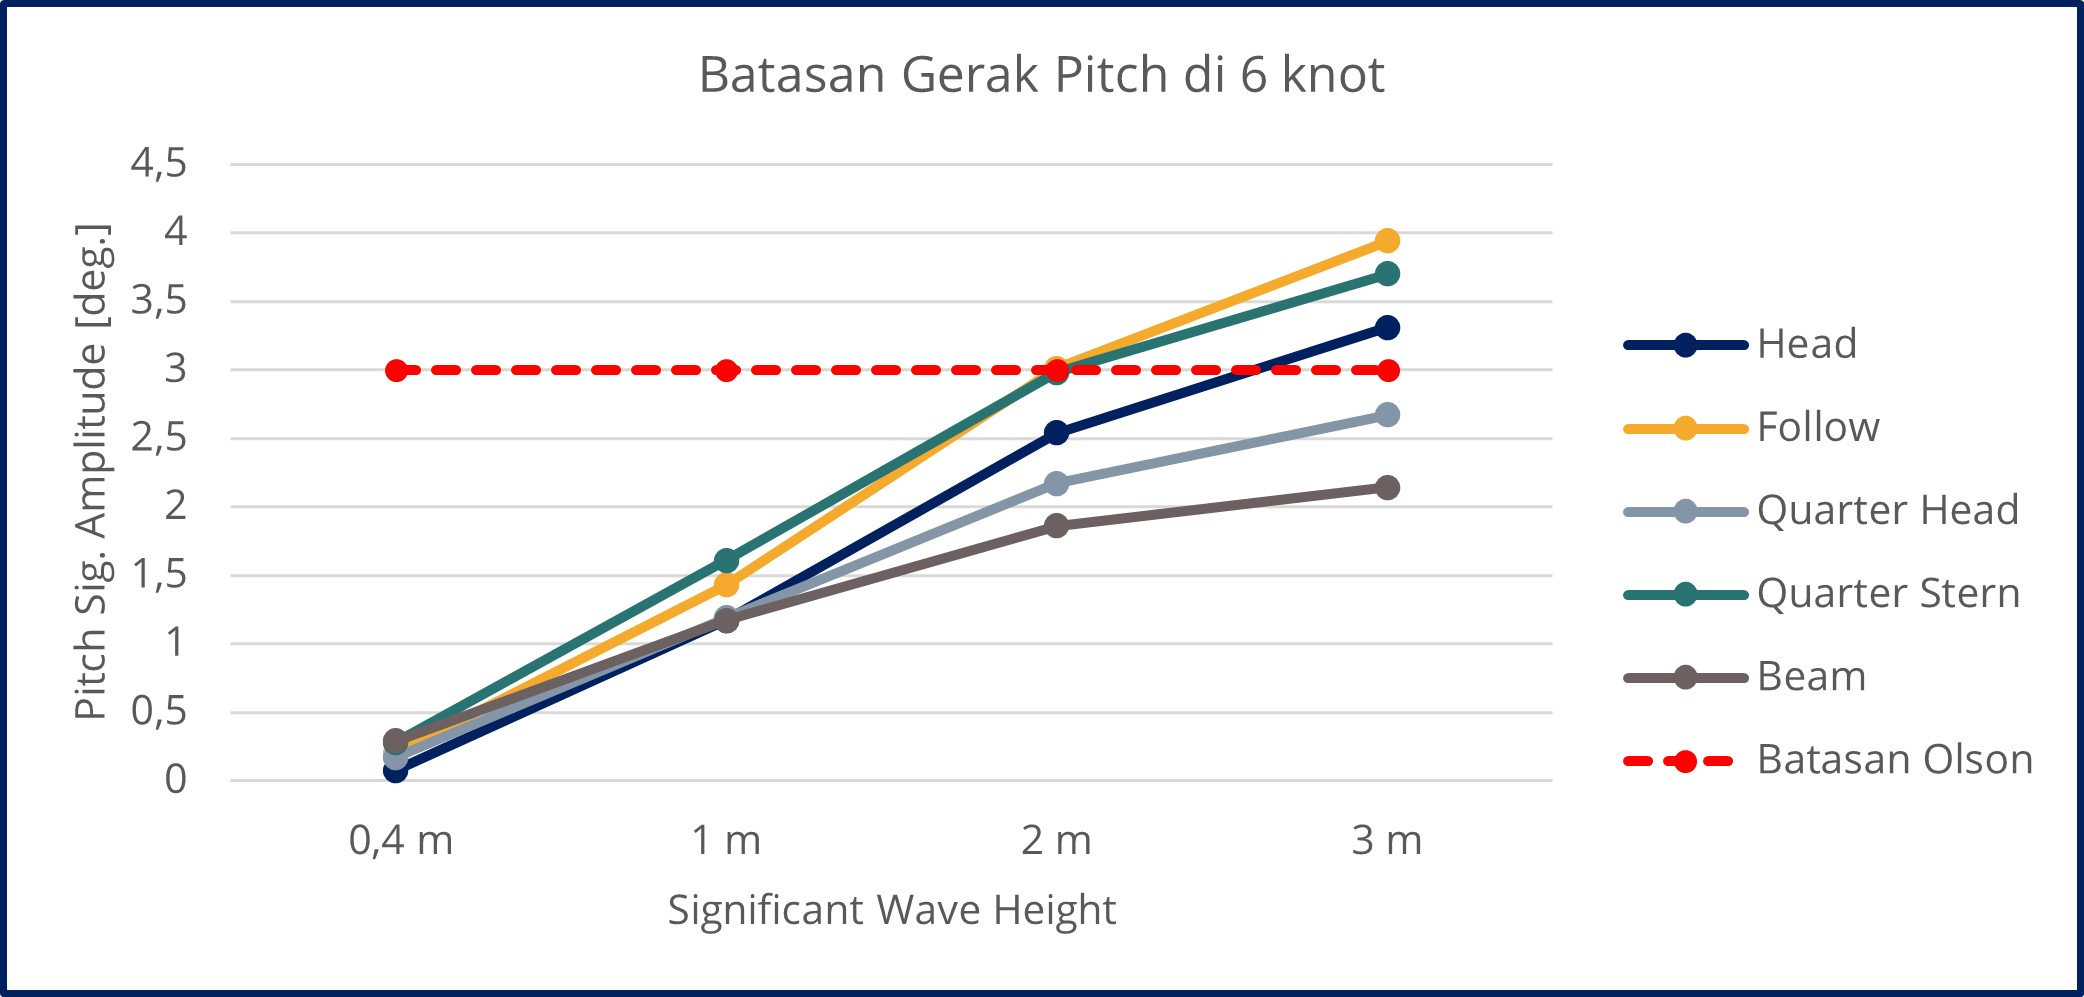
\includegraphics[width=\textwidth]{grafik/uji-pitch-spob.jpg}
    \end{subfigure}
    \hfill  % This adds horizontal spacing between images
    \begin{subfigure}{0.48\textwidth}
        \centering
        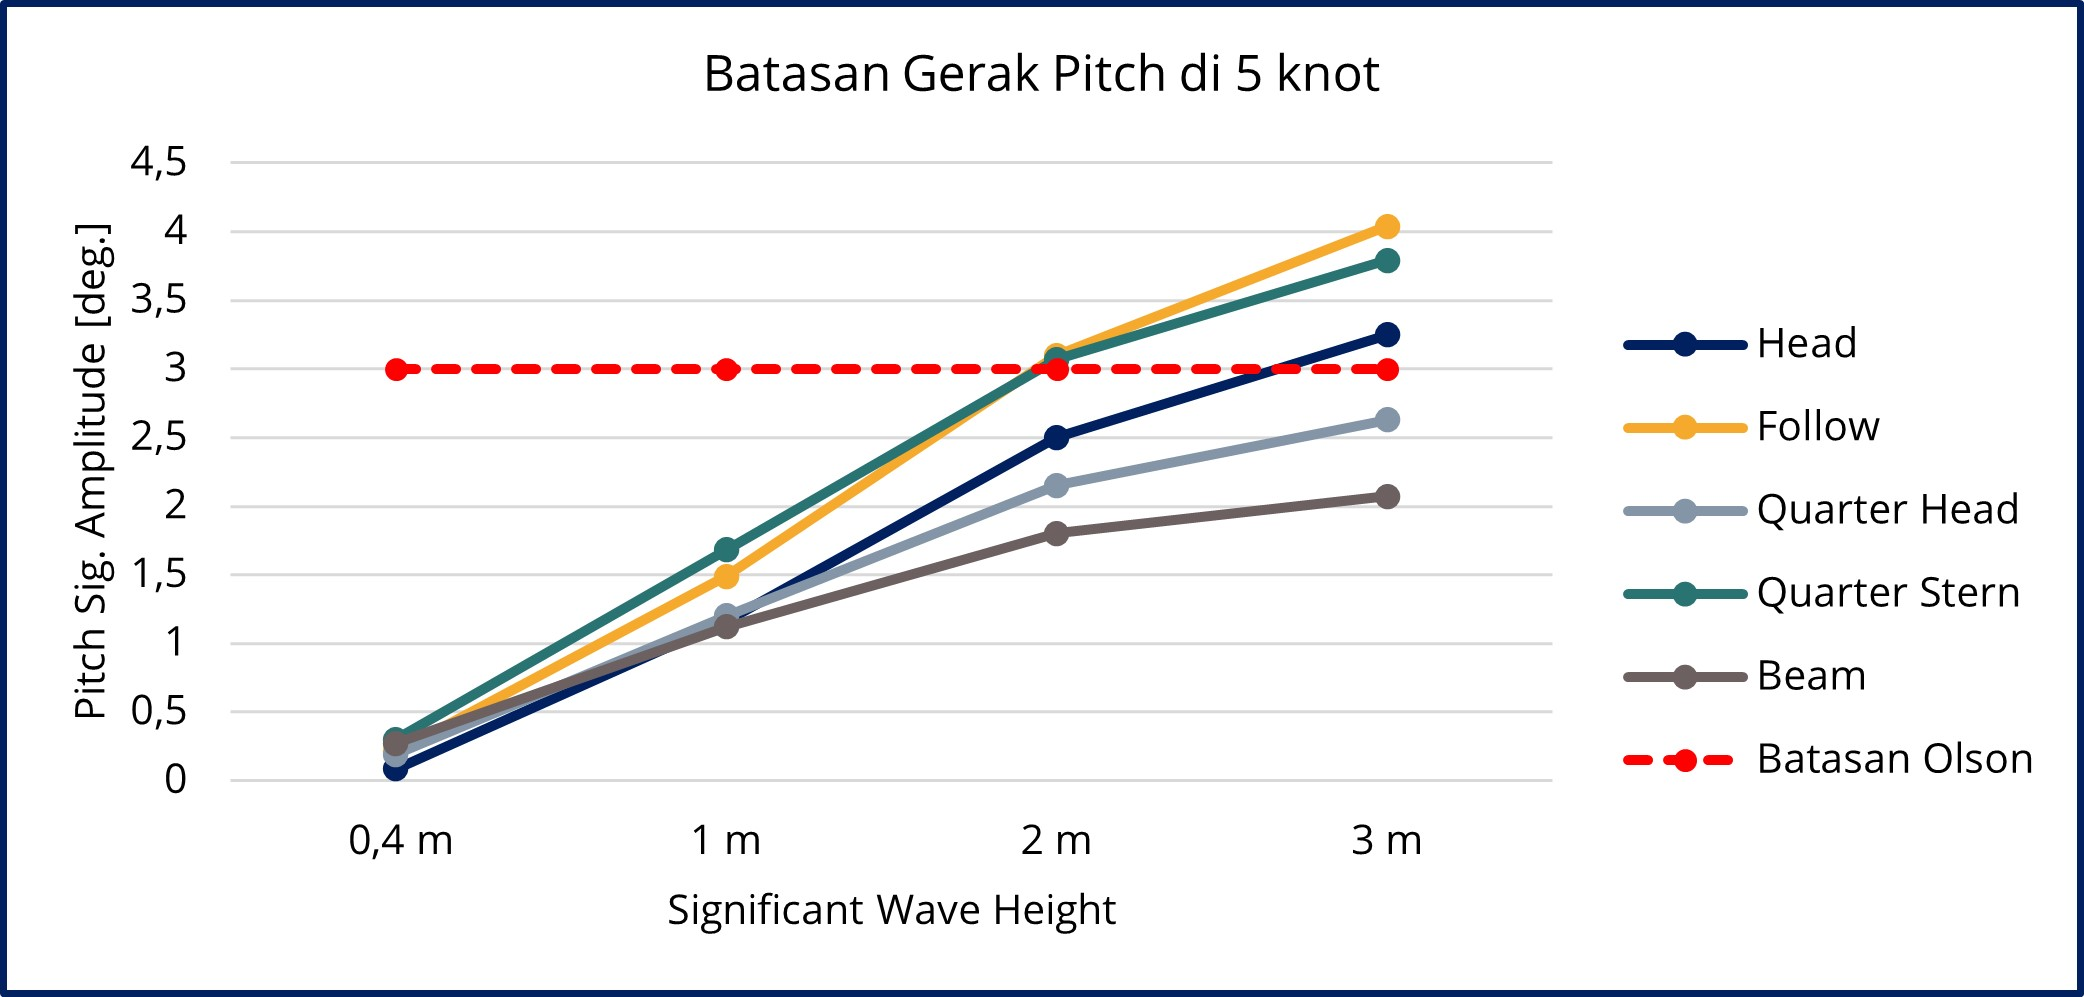
\includegraphics[width=\textwidth]{grafik/uji-pitch-spob2.jpg}
    \end{subfigure}
    \caption{Hasil Uji Gerak \emph{Pitch} Kapal saat ini}
    \label{fig:uji-pitch-spob}
\end{figure}

\begin{figure}[!ht]
    \centering
    \begin{subfigure}{0.48\textwidth}
        \centering
        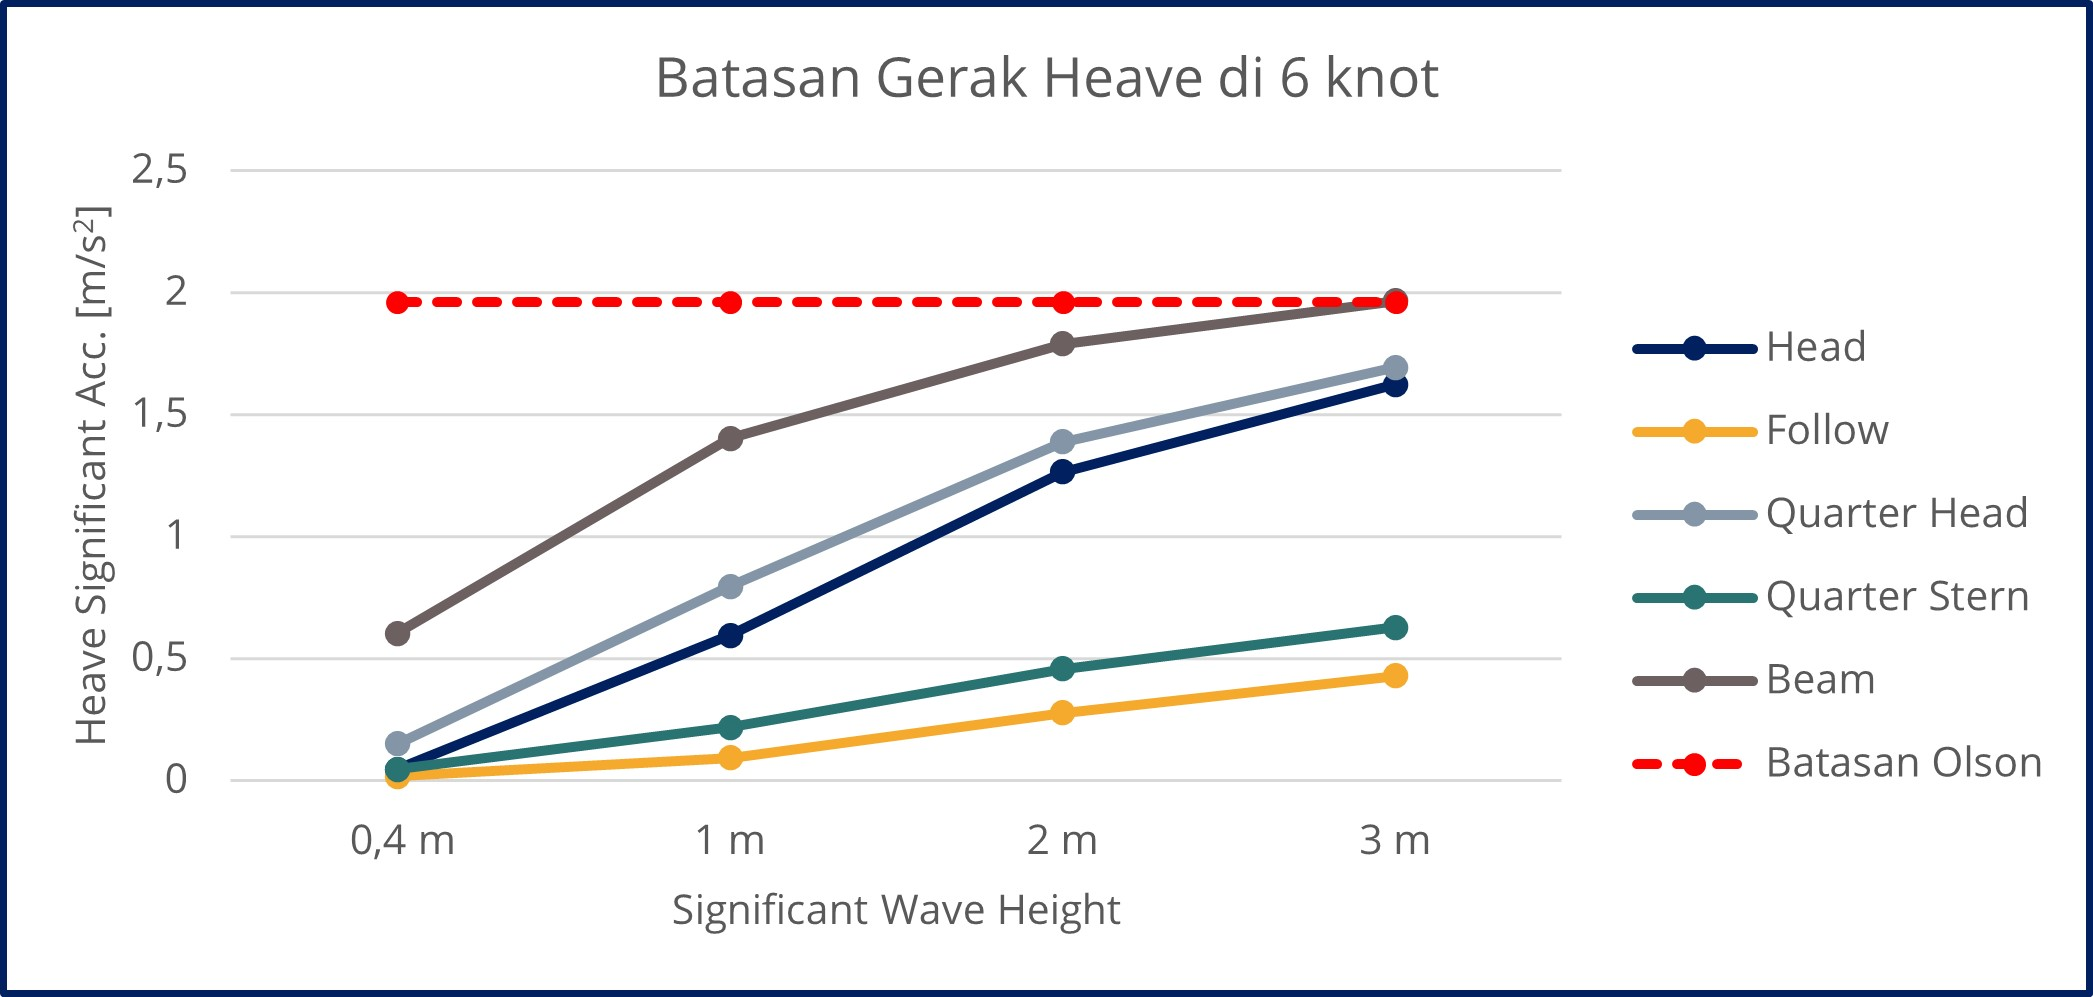
\includegraphics[width=\textwidth]{grafik/uji-heave-spob.jpg}
    \end{subfigure}
    \hfill  % This adds horizontal spacing between images
    \begin{subfigure}{0.48\textwidth}
        \centering
        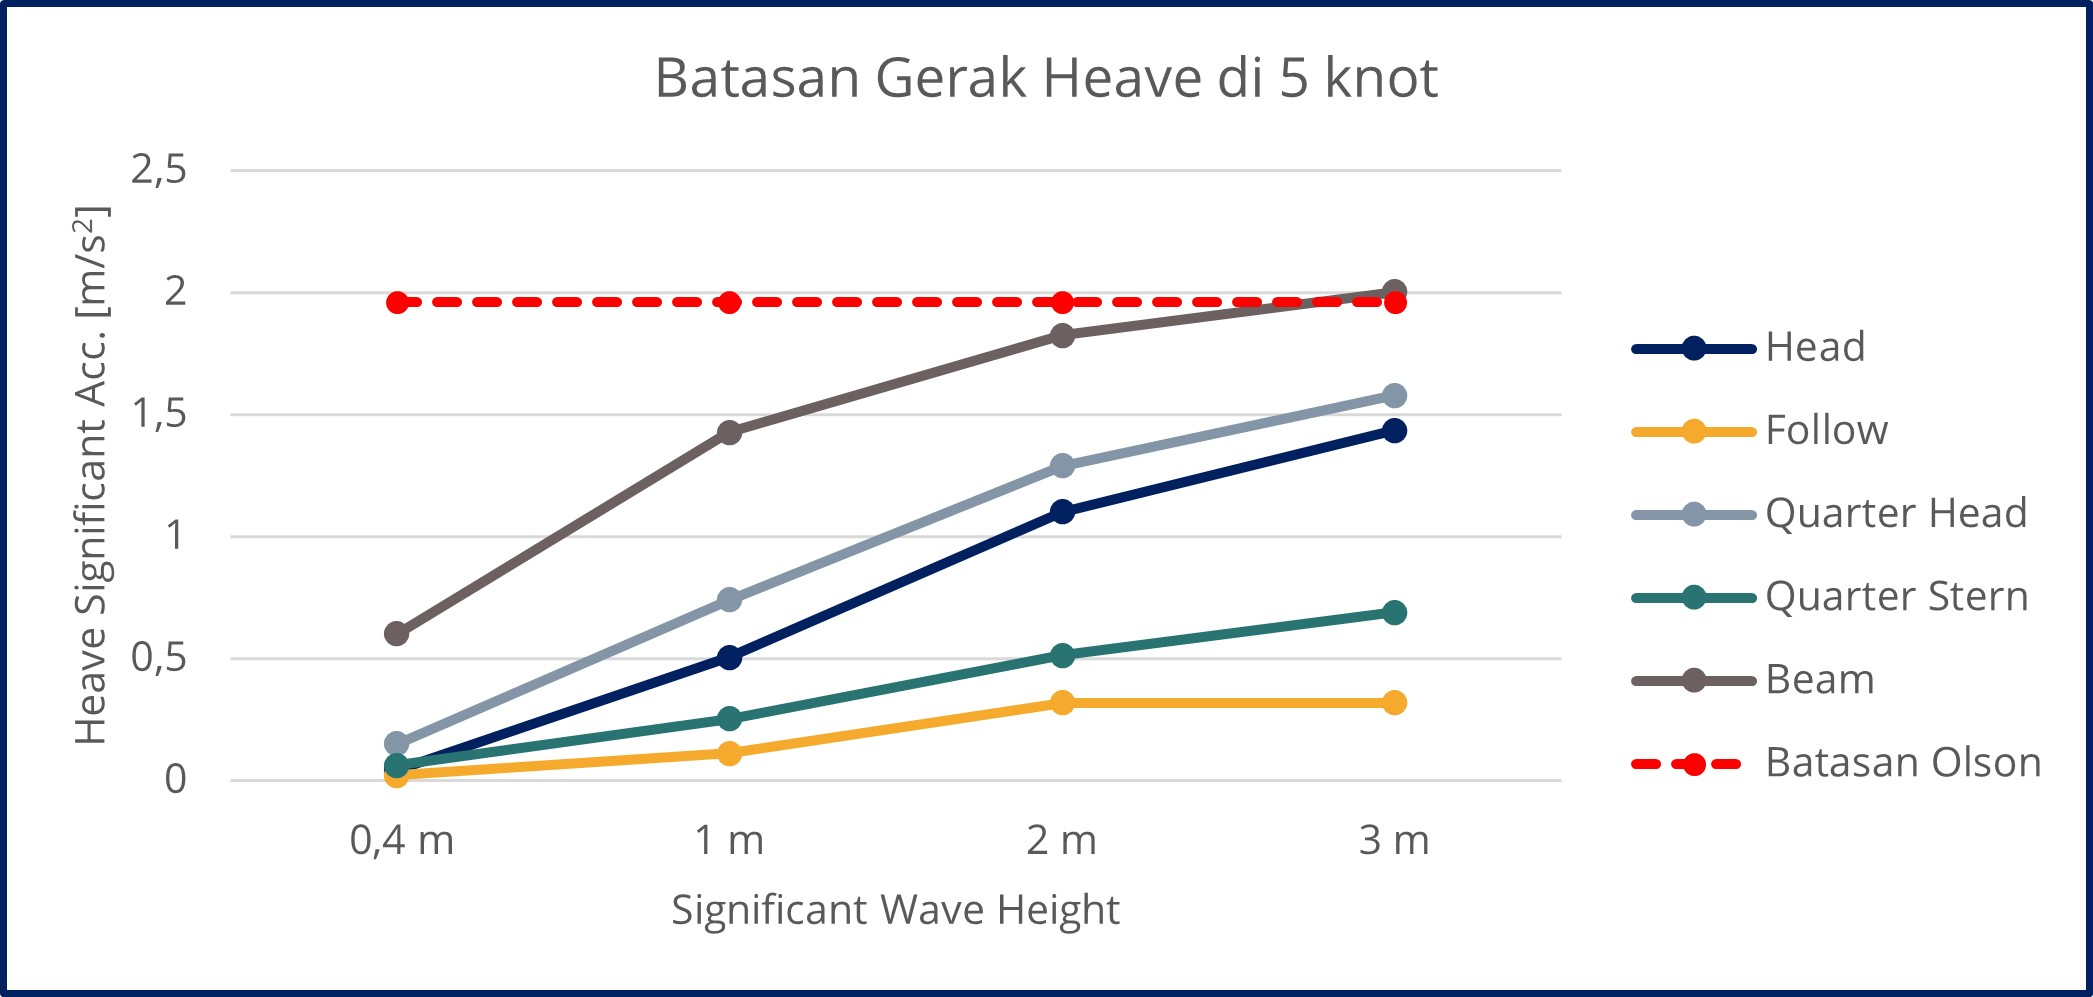
\includegraphics[width=\textwidth]{grafik/uji-heave-spob2.jpg}
    \end{subfigure}
    \caption{Hasil Uji Gerak \emph{Heave} Kapal saat ini}
    \label{fig:uji-heave-spob}
\end{figure}

\begin{figure}[!ht]
    \centering
    \begin{subfigure}{0.48\textwidth}
        \centering
        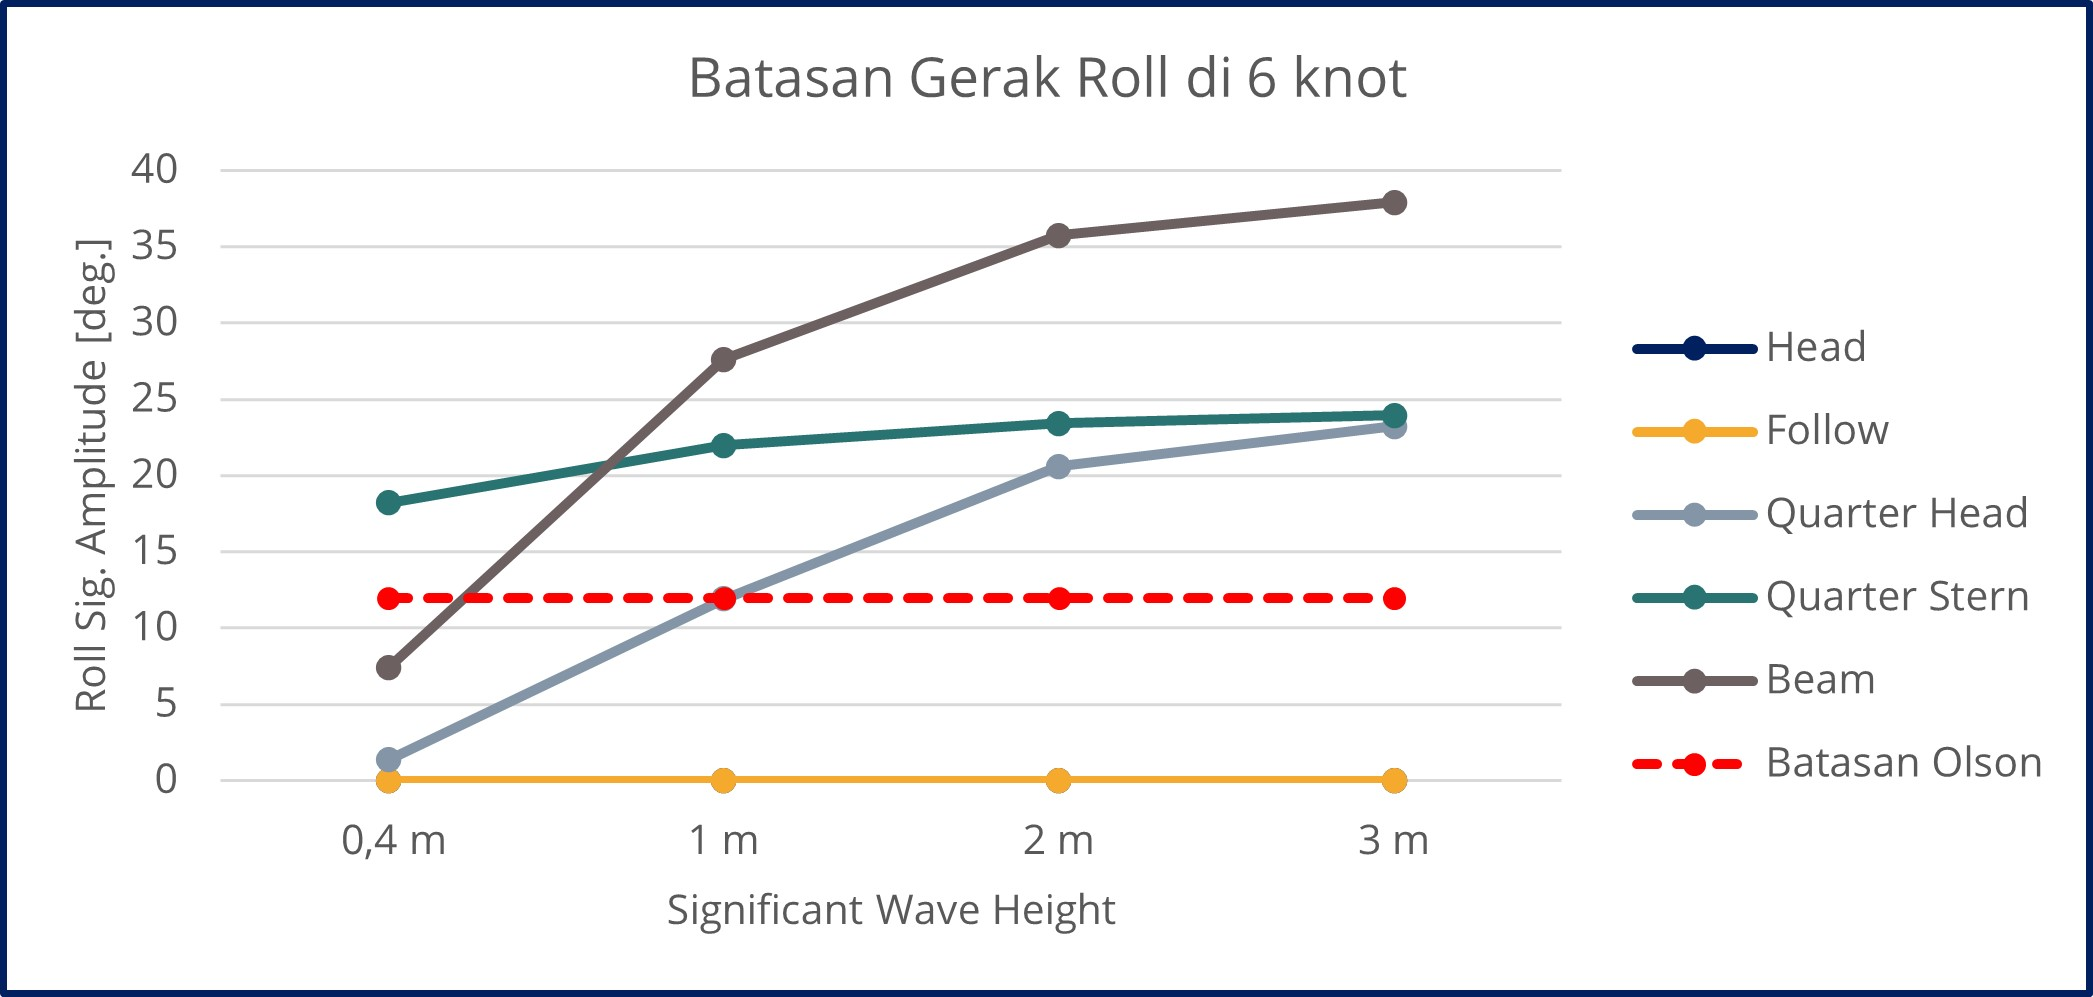
\includegraphics[width=\textwidth]{grafik/uji-roll-spob.jpg}
    \end{subfigure}
    \hfill  % This adds horizontal spacing between images
    \begin{subfigure}{0.48\textwidth}
        \centering
        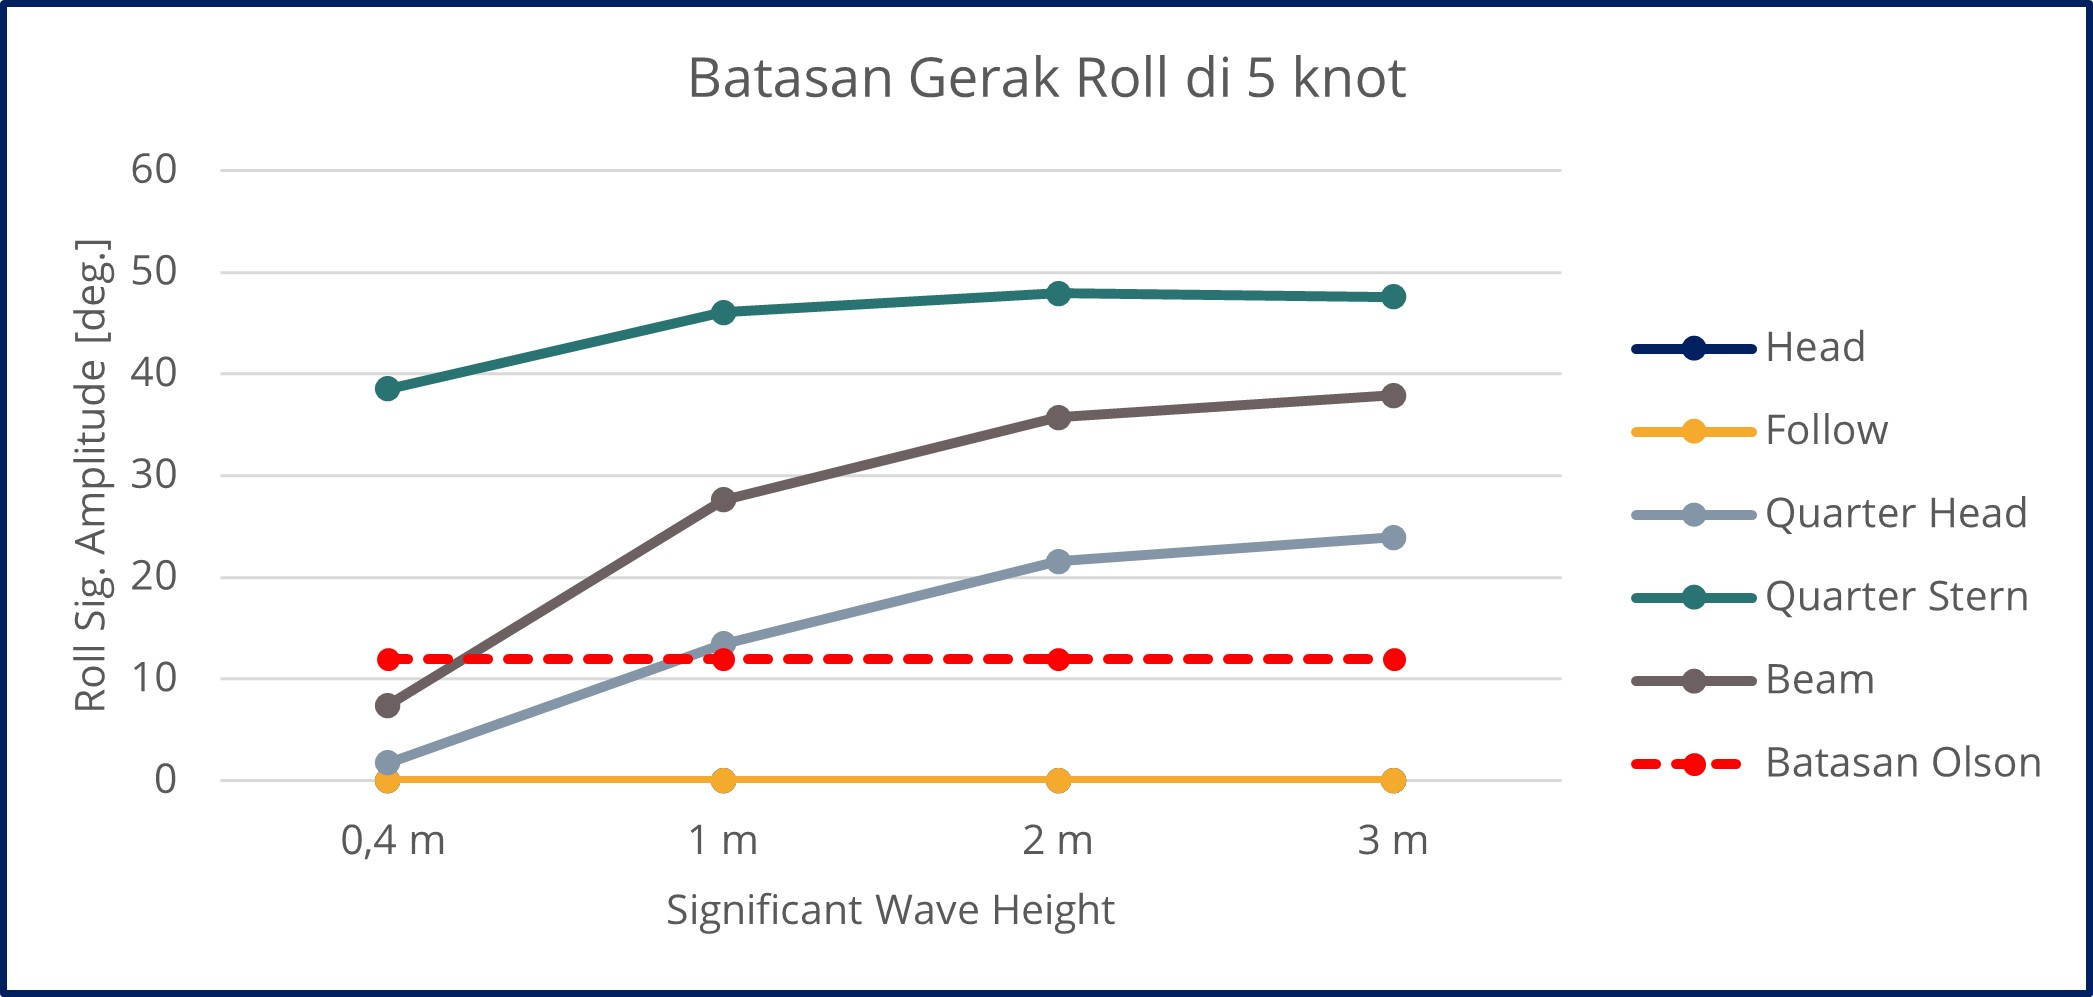
\includegraphics[width=\textwidth]{grafik/uji-roll-spob2.jpg}
    \end{subfigure}
    \caption{Hasil Uji Gerak \emph{Roll} Kapal saat ini}
    \label{fig:uji-roll-spob}
\end{figure}

Berdasarkan hasil uji \emph{seakeeping} yang dapat dilihat pada gambar \ref{fig:uji-pitch-spob} hingga \ref{fig:uji-roll-spob} terlihat pada beberapa arah kedatangan gelombang kapal yang ada saat ini hanya mampu beroperasi pada ketinggian gelombang signifikan 1 meter. Batasan ini yang akan dijadikan dasar simulasi persediaan BBM.

\subsection{Hasil Simulasi Pemasokan}
\label{subsec:simul-existing}

Simulasi dilakukan untuk mencari berapa permintaan BBM yang tidak terpenuhi, hingga biaya tahunan yang saat ini digunakan. Interaksi antara gelombang dengan kemampuan layar kapal akan memunculkan keadaan dimana persediaan BBM yang ada disetiap titik sudah habis namun tidak dapat dilakukan pemasokan, Hal ini yang ingin dipotret dan dijadikan sebagai masalah utama dalam penelitian ini.

\begin{table}[!ht]
    \centering
    \label{table:summary-stat-existing}
    \caption{Tabel Ringkasan Statistik Simulasi}
    \begin{tabular}{|c|c|c|c|c|c|}
    \hline
    \rowcolor[HTML]{F5AA2D} 
    Variabel                  & Satuan        & Min   & Mean  & Max    & Std.   Dev. \\ \hline
    Kekurangan   Bensin       & kiloliter     & 0     & 24,78 & 100,13 & 20,54       \\ \hline
    Kekurangan   Minyak Tanah & Kiloliter     & 0     & 112   & 245    & 57,86       \\ \hline
    Kekurangan   Solar        & kiloliter     & 0     & 1,1   & 17     & 3,01        \\ \hline
    Biaya   Tahunan           & Juta   Rupiah & 7.332 & 8.310 & 9.401  & 389,77      \\ \hline
    Public   Cost             & Juta   Rupiah & 0     & 2.882 & 7.187  & 444,5       \\ \hline
    \end{tabular}
\end{table}

Setelah dilakukan ternyata didapatkan hasil bahwa kemungkinan terjadinya permintaan BBM yang tidak terpenuhi masih sangat besar khususnya minyak tanah. Rata-rata ekspektasi biaya publik yang muncul sebesar 2,8 miliar rupiah.